\section{Vector Fields on Manifolds}
A \textbf{vector field} is a map $X:M \to TM$ such that $X(p) \in T_pM$ for all $p \in M$. We often write $X_p$ for $X(p)$. 
More generally, a vector field on $M$ is a section of the map $\pi:TM \to M$. Intuitively, the section gives a well-defined rule of assigning each $p \in M$ to an element of $T_pM \in TM$. 
\begin{figure}[h]
    \centering
    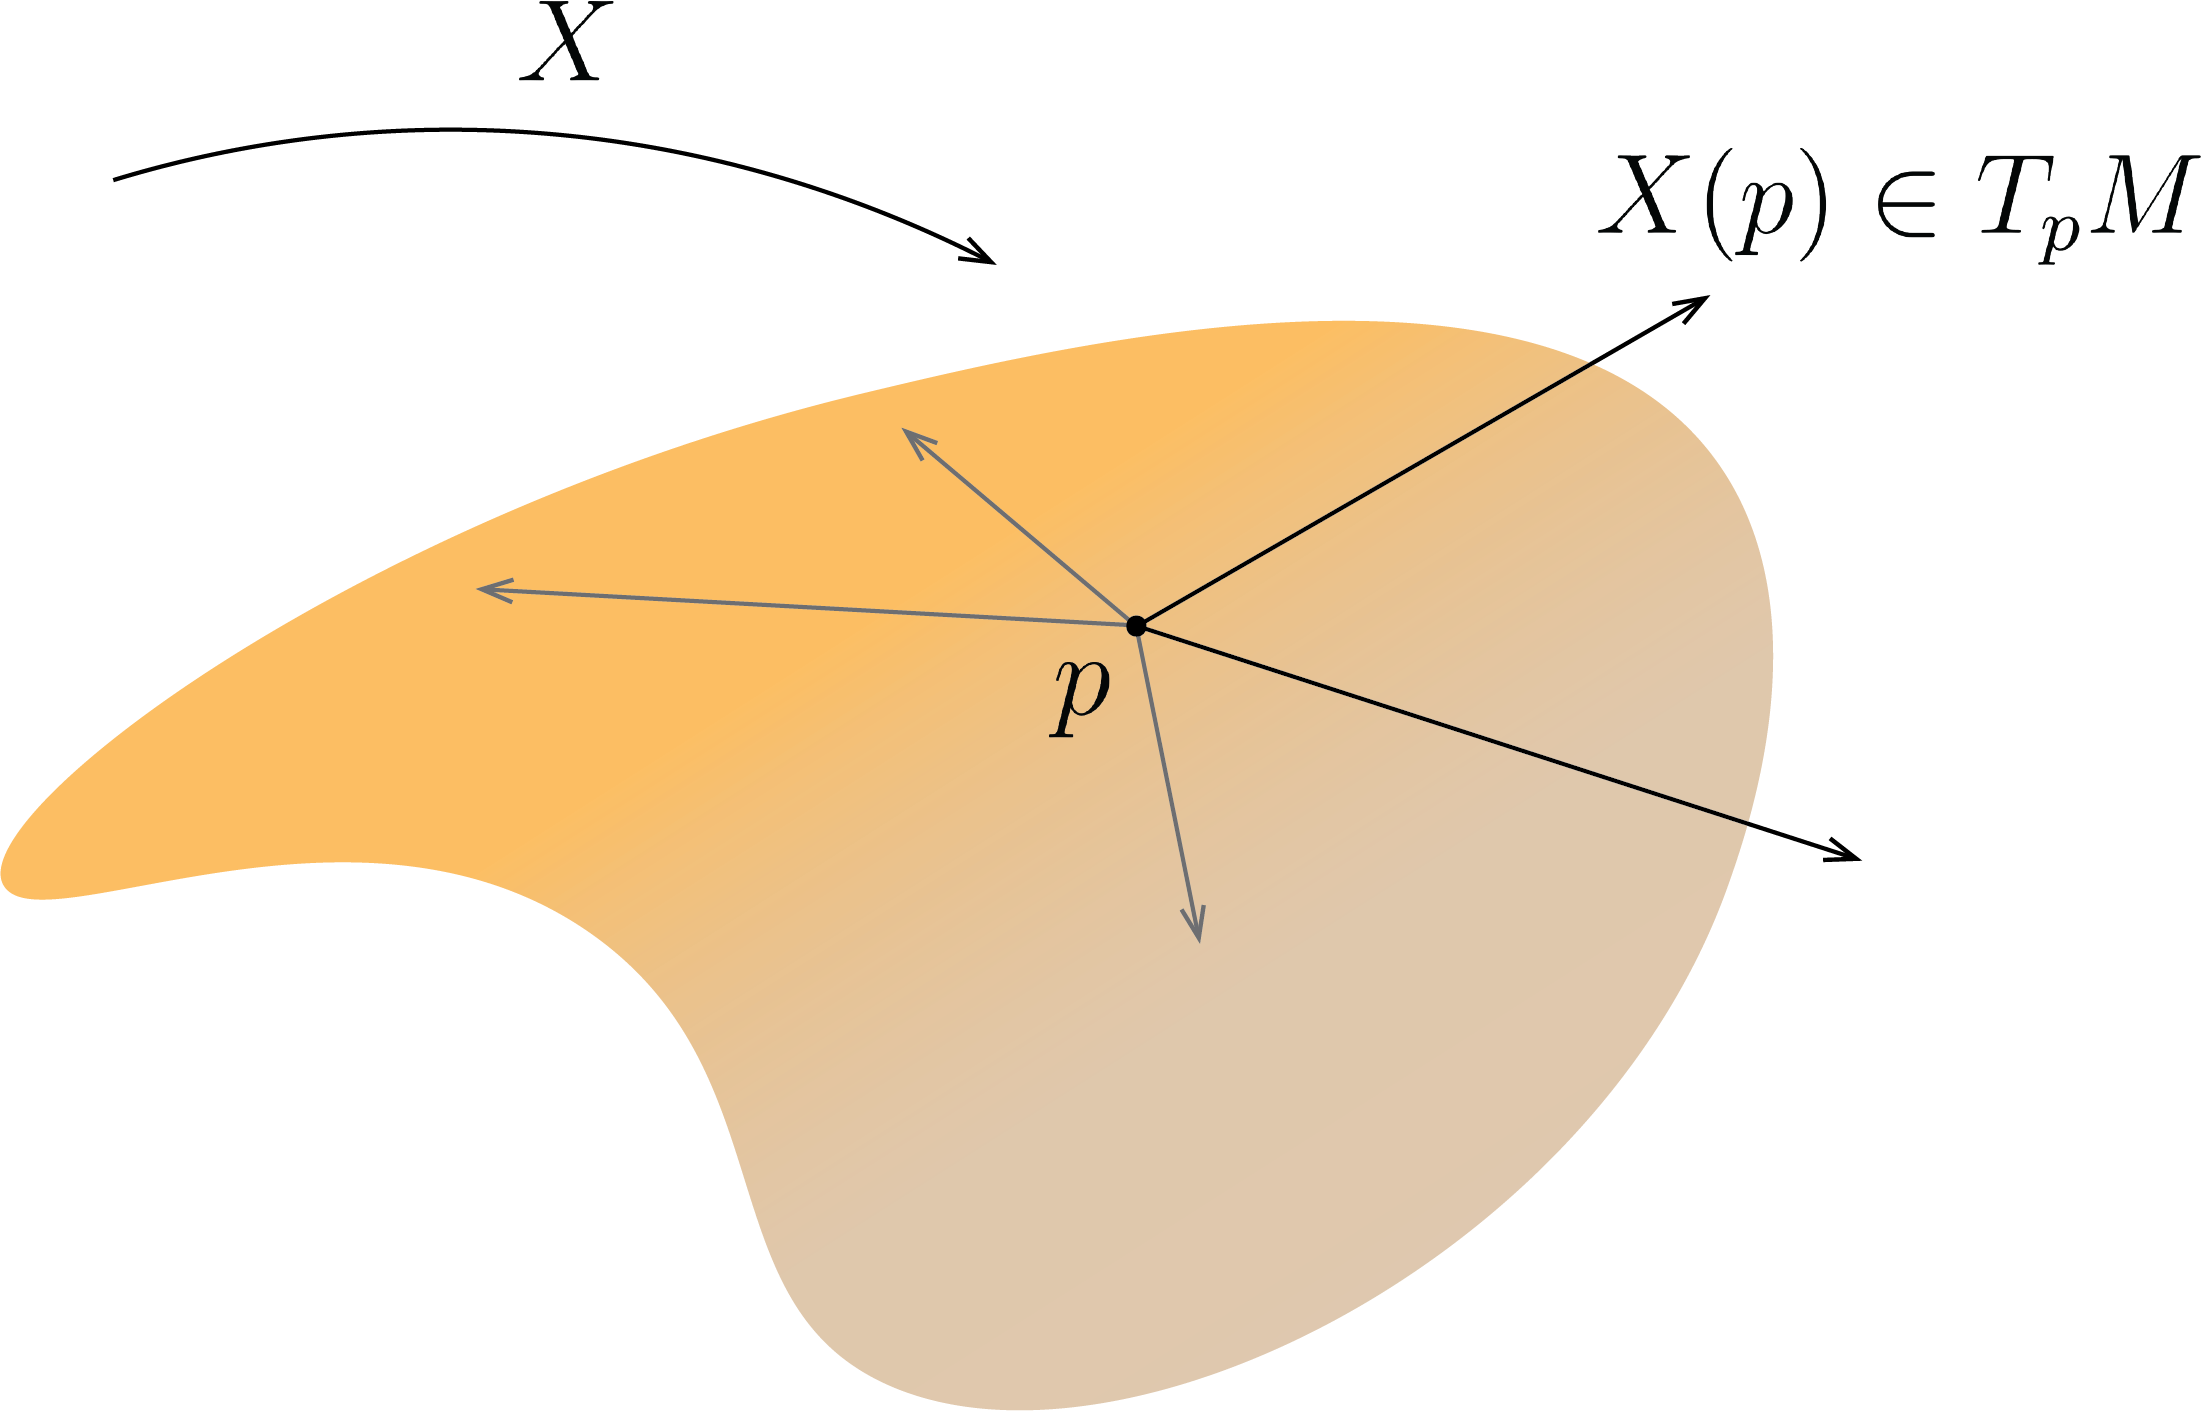
\includegraphics[scale=0.4]{figure/VectorFieldSection.png}
    \caption{There are many tangent vectors in $T_pM$, a vector field picks a unique one so that the map is well-defined. }
\end{figure}

It would be wise to review the smooth structure for $TM$. Recall that $TM = \bigsqcup_{p \in M}T_pM$ and $\pi:TM \to M$ is given by $\pi(p,v) = p$, where $v \in T_pM$. $TM$ is a $2n$-dimensional smooth manifold with the smooth structure 
$$\{(\pi^{-1}(U), \widetilde{\phe}: (U,\phe=(x^i)) \text{ a smooth chart for }M \}, $$ where 
$$\widetilde{\phe}\br{v^i \dvBase{x^i}{p}}
  = \br{x^1(p),\cdots,x^n(p),v^1,\cdots,v^n}.$$
The coordinates $(x^i, v^i)$ are called the \textit{natural coordinates} on $TM$. 

%\noindent \fbox{\Large{\textsc{Local Behavior}}} \\~\\
Given a vector field $X$ and a chart $(U,\phe)$, we can write
$$ X_p = X^i(p) \pdv{}{x^i}\bigg|_p $$
for some functions $X^i:U \to \R$ called the component functions of $X$. 
\begin{proposition}
    A vector field $X:M \to TM$ is smooth if and only if for every chart the component functions are smooth. 
\end{proposition}
\begin{proof}
    We only need to prove the smoothness of the coordinate representation $\hat{X}$. Let $(U,\phe=(x^i))$ be a smooth chart on $M$ and $(\pi^{-1}(U), \widetilde{\phe})$ be the corresponding smooth chart on $TM$.  
    Then 
    \begin{align*}
    \hat{X}(\phe(p)) &= \widetilde{\phe} \circ X \circ \phe^{-1}(\phe(p)) \\
    &= \widetilde{\phe} \circ X (p) \\
    &= \widetilde{\phe}\br{X^i(p) \pdv{}{x^i}\bigg|_p} \\
    &= \br{x^1(p),\cdots,x^n(p),X^1(p),\cdots,X^n(p)}.
    \end{align*}
    It follows that $X$ is smooth if and only if each component $X^i$ is smooth. 
\end{proof}
\begin{example}
    If $(U,(x^i))$ is a smooth chart on $M$, then 
    $$p \mapsto \dvBase{x^i}{p}$$ determines a vector field on $U$. 
\end{example}
\begin{example}[(Euler's Homogeneous Function Theorem)]
    Let $c \in \R$, let $f:\R^n \setminus \{0\} \to \R$ be a smooth function such that $f(\lam x) = \lam^c f(x)$\footnote{Such a function is called \textit{positively homogeneous} of degree $c$.} for all $\lam > 0$ and $x \in \R^n \setminus \{0\}$. Let $V$ be the \textit{Euler vector field} on $\R^n$ given by 
    $$V_x = x^1\dvBase{x^1}{x} + \cdots + x^n\dvBase{x^n}{x}.$$ Prove that $Vf = cf$. 
\end{example}

Let $\frakX(M)$ denote the set of all smooth vector fields. This is naturally a $\R$-vector space where
\begin{itemize}
    \item $(X+Y)_p = X_p + Y_p$ for all $X,Y \in \frakX(M)$,
    \item $(aX)_p = aX_p$ for all $a \in \R, X \in \frakX(M)$. 
\end{itemize}
Given $X \in \frakX(M)$ and $f \in C^\infty(M)$, we can also define $fX \in \frakX(M)$ by 
$(fX)_p = f(p)X(p). $

\begin{proposition}
Let $M$ be a smooth manifold. 
\begin{enumerate}
    \item If $X,Y \in \frakX(M)$ and $f,g \in C^\infty(M)$, then $fX+gY \in \frakX(M)$. 
    \item $\frakX(M)$ is a module over $C^\infty(M)$. 
\end{enumerate}
\end{proposition}
\begin{proof}
    \begin{enumerate}
    \item Let $p \in M$, then 
    \begin{align*}
    (fX+gY)(p) &= f(p)X(p) + g(p)Y(p) \\
    &= f(p)X^i(p)\dvBase{x^i}{p} + g(p)Y^i(p)\dvBase{x^i}{p}
    \end{align*}
    is clearly smooth vector field. 
    \item Recall that a left $C^\infty(M)$-module $\frak{X}(M)$ consists of an abelian group $\frak{X}(M)$ and a left action $\cdot: C^\infty(M) \times \frak{X}(M) \to \frak{X}(M)$. 
    It is easily seen that $C^\infty(M)$ is a ring and $\frak{X}(M)$ is an abelian group, thus we check that $\cdot$ is an action. 
    \begin{itemize}
    \item Let $1$ denote the identity function in $C^\infty(M)$, then $$(1 \cdot X)_p = 1(p)X(p) = X(p)$$ for all $p \in M$. 
    \item Let $f,g \in C^\infty(M)$, then 
    \begin{align*}
    [(fg)\cdot X]_p &= f(p)g(p)X(p)
    = f(p)[g(p)X(p)] = [f \cdot (g \cdot X)]_p.
    \end{align*}
    \end{itemize}
    \end{enumerate}
\end{proof}

\begin{definition}
    If $M$ is a smooth manifold and $A \subset M$, a \textit{vector field along} $A$ is a continuous map $X:A \to TM$ satisfying $\pi \circ X = \id_A$.
    We call it a \textit{smooth vector field along} $A$ if for each $p \in A$, there is a neighborhood $V$ of $p$ in $M$ and a smooth vector field $\widetilde{X}$ on $V$ that agrees with $X$ on $V \cap A$. 
\end{definition}
\begin{lemma}[extension lemma for vector fields]
    Let $M$ be a smooth manifold with or without boundary, and let $A \subseteq M$ be a closed subset. Suppose $X$ is a smooth vector field along $A$. Given any open subset $U$ containing $A$, there exists a smooth global vector field $\tilde{X}$ on $M$ such that $\left.\widetilde{X}\right|_A=X$ and $\operatorname{supp} \widetilde{X} \subseteq U$.
\end{lemma}
\begin{proof}
    The proof uses the standard smooth structure of $TM$ and essentially follows the proof of the extension lemma of a smooth function. The idea is to "pull back" from $\R^{2n}$ to $TM$ using the diffeomorphism $\widetilde{\phe}$. 
    
    We begin by recalling some notations in the construction of the smooth structure on $TM$. If $(U, \phe)$ is a smooth chart on $M$ with coordinates $(x^1, \cdots, x^n)$ and $\pi:TM \to M$ given by $\pi(p,v) = p$, then $(\pi^{-1}(U), \widetilde{\phe})$ is a smooth chart on $TM$, where 
    $$ \widetilde{\phe}\br{v^i \pdv{}{x^i}\bigg|_p} = 
        (x^1(p), \cdots, x^n(p), v^1, \cdots, v^n). $$

    Let $p \in A$, then there is an open neighborhood $W_p$ of $p$ such that there exists a smooth vector field $Y:W_p \to TM$ with $Y|_{W_p \cap A} = X|_{W_p \cap A}$. Without loss of generality we may assume that $W_p$ is the domain of a smooth chart $(W_p,\phe)$ for $M$, Thus $(\pi^{-1}(W_p), \widetilde{\phe})$ is a smooth chart for $TM$.
    
    Because $\{W_p\}_{p \in A}$ is an open cover of $A$, by the gluing lemma, there exists a unique smooth map $Z:A \to TM$ such that  
    $$ Z_{W_p \cap A} = Y|_{W_p \cap A} = X|_{W_p \cap A} \quad \text{for every }p \in A, $$
    thus $X:A \to TM$ is a smooth map. Since $\widetilde{\phe}:\pi^{-1}(W_p) \to \widetilde{\phe}(\pi^{-1}(W_p)) \subset \R^{2n}$ is a diffeomorphism, 
    the composition $\widetilde{\phe} \circ X := f:A \to \R^{2n}$ is smooth.
    
    Since $\pi^{-1}(W_p)$ consists of all the tangent vectors at each point of $W_p$ and $Y$ is a vector field, we have $Y(W_p) \subset \pi^{-1}(W_p)$. Thus $\widetilde{f}_p := \widetilde{\phe} \circ Y: W_p \to TM$ is a smooth map. By replacing $W_p$ by $W_p \cap U$, we may assume that $W_p \subset U$. 
    Now the family $\{W_p\}_{p \in A} \cup \{M \setminus A\}$ is an open cover of $M$, so there exists a smooth partition of unity $\{\psi_p\}_{p\in A} \cup \{\psi_0\}$ subordinate to this cover such that 
    \begin{itemize}
        \item $\supp \psi_p \subset W_p$,
        \item $\supp \psi_0 \subset M \setminus A$,
        \item $\{\supp \psi_p\}$ is locally finite. 
        \item $\bigcup_{p \in A}\supp \psi_p \subset U$.
    \end{itemize}
    The product $\psi_p \widetilde{f}_p$ is smooth on $W_p$ and admit a smooth extension to all of $M$ since $\supp \psi_p \subset W_p$. Define 
    $\widetilde{f}:M \to \R^{2n}$ by
    $$\widetilde{f}(x) = \sum_{p \in A} \psi_p(x) \widetilde{f}_p(x), $$
    which is a finite sum due to the local finiteness of $\{\supp \psi_p\}$, thus $\widetilde{f}$ is a smooth map. 

    Define $\widetilde{X}:M \to TM$ by 
    $$ \widetilde{X}(x) = \widetilde{\phe}^{-1} \circ \widetilde{f}(x),$$
    then 
    \begin{itemize}
    \item $\widetilde{X}$ is smooth since it is a composition of smooth maps, and
    $$\widetilde{X}(x) = Y(x) \in T_x M, $$
    so that $\widetilde{X}(x)$ is a smooth vector field. 
    \item If $x \in A$, then 
    \begin{align*}
        \widetilde{\phe}^{-1} \circ \widetilde{f}(x) 
        &= \widetilde{\phe}^{-1}\br{\sum_{p \in A}\psi_p(x)\widetilde{f}_p(x)} \\
        &= \widetilde{\phe}^{-1}\br{\sum_{p \in A}\psi_p(x) f(x)} \\
        &= \widetilde{\phe}^{-1}\br{f(x) \sum_{p \in A}\psi_p(x)} \\
        &= \widetilde{\phe}^{-1}(f(x)) \\
        &= \widetilde{\phe}^{-1}(\widetilde{\phe} \circ X(x)) \\
        &= X(x),
    \end{align*}
    hence $\widetilde{X}|_A = X|_A$.
    \item By the coordinate representation of $\widetilde{\phe}$, we have $\widetilde{\phe}^{-1}(0) = 0$, thus
    $$\supp \widetilde{X} = \supp \widetilde{\phe}^{-1} \circ \widetilde{f} \subset \supp \widetilde{f} = \bigcup_{p \in A}\supp \psi_p \subset U, $$
    \end{itemize}
    completing the proof. 
\end{proof}
\subsection{Local and Global Frames}
Fix a point $p$ in a smooth chart $(U,\phe)$, then $X_p \in T_p M \simeq \R^n$. Now we consider the case when there are finitely many vector fields. Let $X_1,\cdots,X_k$ be a list of vector fields defined on some $A \subset M$. This list  
\begin{itemize}
    \item is called \textit{linearly independent} if the list $X_1|_p, \cdots, X_k|_p$ is linearly independent in $T_pM$ for each $p \in A$. 
    \item said to \textit{span} the tangent bundle if 
    $\Span \cBr{X_1|_p, \cdots, X_k|_p} = T_pM$ for each $p \in A$. 
\end{itemize}
\begin{definition}[frame]
    Let $M$ be a smooth $n$-manifold.
    A \textit{local frame} for $M$ is a list of vector fields $(E_1,\cdots,E_n)$ defined on an open $U \subset M$ that is linearly independent and spans the tangent bundle, equivalently, 
    $E_1|_p,\cdots,E_n|_p$ is a basis for $T_pM$ at each $p \in U$. It is called a \textit{global frame} if $U=M$. 
    \begin{itemize}
        \item $(E_1,\cdots,E_n)$ is called a \textit{smooth frame} if each $E_i$ is smooth. 
        \item For $k \in \N$, $(E_1,\cdots,E_k)$ defined on $A \subset \R^n$ is called \textit{orthonormal} if for each $p \in A$, $E_1|_p, \cdots, E_k|_p$ are orthonormal w.r.t. the Euclidean inner product. 
    \end{itemize} 
    We denote a frame $(E_1,\cdots,E_n)$ by $(E_i)$. 
\end{definition}
\begin{figure}[h]
    \centering
    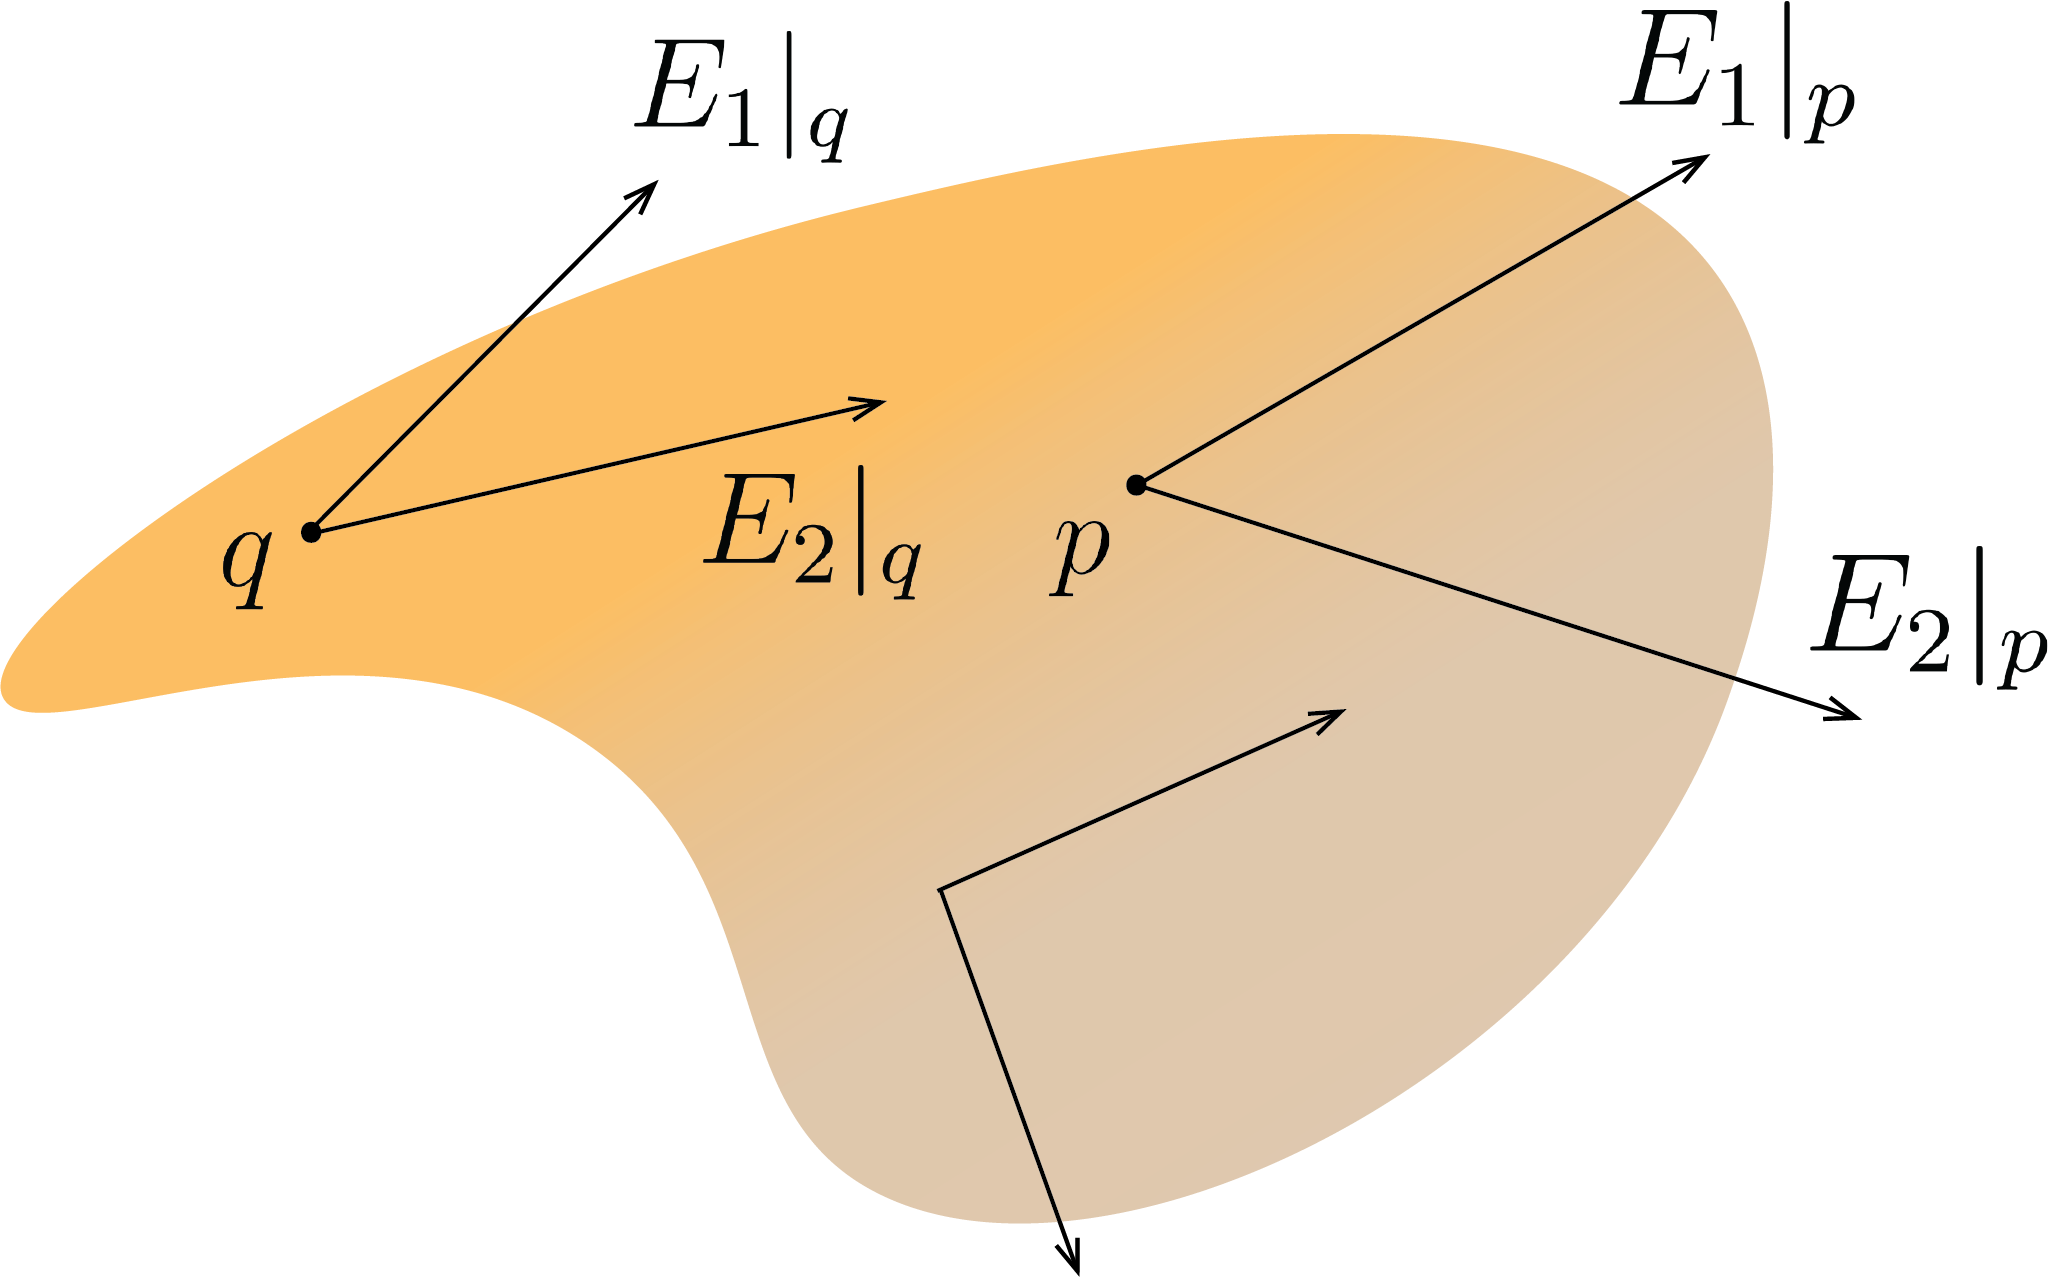
\includegraphics[scale=0.5]{figure/frame.png}
\end{figure}






\begin{example}
    The standard coordinate vector fields 
    $$\br{\dvBase{x^1}{p}, \cdots, \dvBase{x^n}{p}}$$ form a smooth global frame for $\R^n$. 
\end{example}



\subsection{Vector Fields as Derivations of $C^\infty(M)$}
A derivation of $C^\infty(M)$ is a map $D:C^\infty(M) \to C^\infty(M)$ such that 
$$D(fg) = fD(g) + gD(f) \quad \text{for all }f,g \in C^\infty(M). $$
This looks like the derivation (studied in tangent space) without referring to a point. 

If $X \in \frakX(M)$ and $f \in C^\infty(M)$, we define
\begin{align*}
    Xf:M &\to \R \\
    (Xf)(p) &= X_p(f).
\end{align*}
This makes sense since $X_p \in T_pM$, so it acts on any $f \in C^\infty(M)$. It turns out that the smoothness of $X$ and the smoothness of $Xf$ are related. 
\begin{proposition}\label{8.14}
    Let $X:M \to TM$ be a vector field. The following are equivalent:
    \begin{enumerate}
    \item $X$ is smooth.
    \item $Xf$ is a smooth function on $M$ for every $f \in C^\infty(M)$. 
    \item $Xf$ is smooth on $U$ for every open $U \subset M$ and every $f \in C^\infty(U)$. 
    \end{enumerate}
\end{proposition}
\begin{proof}
    (1) $\implies$ (2): Let $X$ be smooth, $f \in C^\infty(M), p \in M$. Choose smooth coordinates $(x^i)$ on a neighborhood $U$ of $p$, then for all $x \in U$, we can write 
    $$ Xf(x) = \br{X^i(x)\dvBase{x^i}{x}}f = X^i(x){\pdv{f}{x^i}}(x). $$
    Since $f \in C^\infty(M)$, $\pdv*{f}{x^i}$ is smooth. Since components $X^i$ are smooth, it follows that $Xf$ is smooth on $U$. Because $U$ is arbitrary, $Xf$ is smooth on $M$. \\
    (2) $\implies$ (3): Let open $U \subset M$ and $f \in C^\infty(U)$. For any $p \in U$, let $\psi$ be a smooth bump function such that $\psi=1$ on a neighborhood of $p$ and $\supp \psi \subset U$. Define $\widetilde{f} = \psi f$, extended to be $0$ on $M \setminus \supp \psi$, then $X\tilde{f}$ is smooth, and $X\tilde{f} = Xf$ in a neighborhood of $p$. \\
    (3) $\implies$ (1): Suppose (3) holds, let $(x^i)$ be a smooth local coordinates on $U \subset M$, we can think of each $x^i$ as a smooth function on $U$. Then 
    $$Xx^i = X^j {\pdv{}{x^j}}(x^i) = X^i, $$
    so each $X^i$ is smooth, hence $X$ is smooth. 
\end{proof}

\begin{proposition}
    A map $D:C^\infty(M) \to C^\infty(M)$ is a derivation if and only if $Df = Xf$ for some $X \in \frak{X}(M)$. 
\end{proposition}
\begin{proof}
    First we show that $X$ induces a derivation. 
    \begin{align*}
    X(fg)(p) &= X_p(fg) = f X_p g + g X_p f \\
    &= f(Xg)(p) + g(Xf)(p),
    \end{align*}
    and $X$ is clearly linear, thus $X:C^\infty(M) \to C^\infty(M)$ is a derivation. \\
    Conversely, we need to construct a vector field $X$ such that $Df = Xf$ for all $f$. Fix an arbitrary $p \in M$, and define 
    $X_p$ by 
    $$X_p f = (Df)(p), $$ then $X_p:C^\infty(M) \to \R$ is a tangent vector. Since $p$ is arbitrary, this defines a vector field $X$. by \textbf{Proposition} \ref{8.14}, $X$ is smooth. 
\end{proof}

\section{Vector Fields and Smooth Maps}
We can map a vector field on $M$ to a vector field on $N$. Let $F:M \to N$ be smooth and $X$ be a vector field on $X$, then the differential of $F$ at $p$ is $dF_p:T_pM \to T_pN$, thus $dF_p(X_p) \in T_pN$. However, this does not necessarily define a vector field on $N$.
\begin{example}
    Let $M = \R^2, N = \R^3, F(x^1,x^2) = (x^1,x^2,0)$, then $dF$ is not surjective, so there is no vector to assign at $q \in N \setminus F(M)$. 
\end{example}
\begin{definition}
    Suppose $F:M \to N$ is smooth and $X$ is vector field on $M$, and suppose there is a vector field $Y$ on $N$ such that for each $p \in M$, $dF_p(X_p) = Y_{F(p)}$, then we say $X$ and $Y$ are \textit{$F$-related}.
\end{definition}

\begin{proposition}
    Suppose $F:M \to N$ is a smooth map between manifolds, $X \in \frak{X}(M) ,Y \in \frak{X}(N)$. Then $X$ and $Y$ are $F$-related if and only if for every $f \in C^\infty(V)$, where $V$ is open in $N$, 
    $$ X(f \circ F) = (Yf) \circ F. $$
\end{proposition}
\begin{proof}
    Let $p \in M$ and $f$ defined in a neighborhood of $F(p)$ be smooth, then 
    $$X(f \circ F)(p) = X_p(f \circ F) = dF_p(X_p)f. $$ We also have 
    $$(Yf) \circ F(p) = (Yf)(F(p)) = Y_{F(p)}f. $$
\end{proof}
\begin{example}
    Let $F(t) = (\cos t, \sin t)$, then $d/dt \in \frak{X}(\R)$ is $F$-related to the vector field $Y \in \frak{X}(\R^2)$ defined by 
    $$Y = x\pdv{}{y} - y\pdv{}{x}. $$
\end{example}
\begin{proof}
    \fbox{From definition}
    To compute $dF_p(X_p)$, we need to plug in an arbitrary $f \in C^\infty(\R^2)$. Thus
    \begin{align*}
    dF_{t_0}\br{\frac{d}{dt}\bigg|_{t_0}}f(t) 
    &= \frac{d}{dt}\bigg|_{t_0} \br{f \circ F}(t) \\
    &= \frac{d}{dt}\bigg|_{t_0} f(\cos t, \sin t) \\
    &= -\sin t_0 {\pdv{f}{x}}(\cos t_0, \sin t_0) + \cos t_0{\pdv{f}{y}}(\cos t_0, \sin t_0), 
    \end{align*}
    and $$Y_{F(t_0)}f = \cos t_0 \pdv{f}{y}\bigg|_{F(t_0)} - \sin t_0 \pdv{f}{x}\bigg|_{F(t_0)} $$
    \fbox{By the above proposition}
\end{proof}
\begin{proposition}
    Suppose $F:M \to N$ is a diffeomorphism. For every $X \in \frak{X}(M)$, there is a unique smooth vector field on $N$ that is $F$-related to $X$. 
\end{proposition}


\section{Lie Brackets}
\begin{definition}
    The \textit{Lie bracket} of $X,Y \in \frak{X}(M)$ is the map
    \begin{align*}
    [X,Y]: C^\infty(M) &\longrightarrow C^\infty(M) \\
    [X,Y](f) &= XYf - YXf.
    \end{align*}
\end{definition}
\begin{lemma} % 8.25
    $[X,Y] \in \frak{X}(M)$. 
\end{lemma}
\begin{proof}
    Just compute
    $$[X,Y](fg) = f[X,Y]g + g[X,Y]f, $$ where $f \in C^\infty(M)$. 
\end{proof}
\begin{example}
    In general, $XY \notin \frak{X}(M)$. If $M=\R^2, X=\pdv*{}{x}, Y=x\pdv*{}{y}, f(x,y)=x, g(x,y)=y$, then 
    \begin{align*}
    &XY(fg) = \pdv{}{x}\br{ {x\pdv{}{y}}(xy) } = 2x, \\
    &fXY(g) + gXY(f) = x\pdv{}{x}\br{ {x\pdv{}{y}}(xy) } + y \pdv{}{x}\br{ x{\pdv{}{y}}(x) } = 
    \end{align*}
\end{example}

\begin{proposition}
    If $X,Y \in \frak{X}(M)$ and $(U,\phe)$ is a smooth chart, then locally
    $$ [X,Y] = \br{X^i \pdv{Y^j}{x^i} - Y^i \pdv{X^j}{x^i}} \pdv{}{x^j}. $$
\end{proposition}

\begin{proposition}[properties of Lie brackets]\label{8.28}
    
\end{proposition}

\subsection*{Pushforwards}
Given $X \in \frak{X}(M)$ and a diffeomorphism $F:M \to N$, the \textit{push forward} of $X$ is the vector field $F_* X \in \frak{X}(N)$ defined by 
$$(F_* X)_q = dF_{F^{-1}(q)}\br{ X_{F^{-1}(q)} }. $$

\begin{lemma}
    If $F:M \to N$ is a diffeomorphism, $X \in \frak{X}(M)$, and $f \in C^\infty(N)$, then 
    $$(F_* X)(f) = X(f \circ F) \circ F^{-1}. $$
\end{lemma}

\begin{corollary}
    If $F:M \to N$ is a diffeo and $X,Y \in \frak{X}(M)$, then 
    $$F_*[X,Y] = [F_*X, F_*Y]. $$
\end{corollary}